\documentclass[aspectratio=169]{beamer}

\usepackage{fontspec}
\usepackage{polyglossia}
\usepackage{color}
\usepackage{listings}
\setdefaultlanguage{russian}
\usepackage{csquotes}
\usetheme{metropolis}
\metroset{background=light}
\metroset{sectionpage=none}
\metroset{numbering=fraction}

\definecolor{ssaublue}{RGB}{77,144,205}
\setbeamercolor{frametitle}{fg=white, bg=ssaublue}
\setbeamercolor{title separator}{fg=ssaublue}

\setmainfont[
    Path = ../fonts/elektratextpro/,
    Extension = .otf,
    UprightFont = elektratextpro,
    BoldFont = elektratextpro_bold,
    ItalicFont = elektratextpro_italic,
    BoldItalicFont = elektratextpro_bolditalic
]{elektratextpro}

\setsansfont[
    Path = ../fonts/elektratextpro/,
    Extension = .otf,
    UprightFont = elektratextpro,
    BoldFont = elektratextpro_bold,
    ItalicFont = elektratextpro_italic,
    BoldItalicFont = elektratextpro_bolditalic
]{elektratextpro}

\setmonofont[
    Path = ../fonts/elektratextpro/,
    Extension = .otf,
    UprightFont = elektratextpro,
    BoldFont = elektratextpro_bold,
    ItalicFont = elektratextpro_italic,
    BoldItalicFont = elektratextpro_bolditalic
]{elektratextpro}

\newfontfamily\cyrillicfont[
    Path = ../fonts/elektratextpro/,
    Extension = .otf,
    UprightFont = elektratextpro,
    BoldFont = elektratextpro_bold,
    ItalicFont = elektratextpro_italic,
    BoldItalicFont = elektratextpro_bolditalic
]{elektratextpro}

\newfontfamily\cyrillicfontsf[
    Path = ../fonts/elektratextpro/,
    Extension = .otf,
    UprightFont = elektratextpro,
    BoldFont = elektratextpro_bold,
    ItalicFont = elektratextpro_italic,
    BoldItalicFont = elektratextpro_bolditalic
]{elektratextpro}

\newfontfamily\cyrillicfonttt[
    Path = ../fonts/elektratextpro/,
    Extension = .otf,
    UprightFont = elektratextpro,
    BoldFont = elektratextpro_bold,
    ItalicFont = elektratextpro_italic,
    BoldItalicFont = elektratextpro_bolditalic
]{elektratextpro}

% Настройка листингов для Beamer
\lstset{
    basicstyle=\ttfamily\footnotesize,
    commentstyle=\color{gray},
    columns=fullflexible,
    keepspaces=true,
    breaklines=false,
    extendedchars=true,
    texcl=true,
    showstringspaces=false
}

\title{CI/CD пайплайн}
\author{Правдин Иван}
\date{24 сентября 2025 г.}

\begin{document}
    \maketitle

    \begin{frame}{Что мы имеем после прошлой лекции}
        \textbf{Наш webhook сервер работает:}
        
        \begin{itemize}
            \item Git push → автоматический деплой
            \item Разные ветки обновляют разные окружения
        \end{itemize}

        \textbf{Но:}

        \begin{itemize}
            \item Изменения вебхук сервера требуют ручного вмешательства
            \item Нет простого доступа к логам скриптов, нет статуса деплоя
        \end{itemize}
    \end{frame}

    \begin{frame}{Индустриальные решения}
        \textbf{В реальных проектах используют готовые платформы:}
        
        \begin{itemize}
            \item \textbf{Jenkins} — самый популярный, self hosted
            \item \textbf{GitHub Actions} — встроен в GitHub, есть бесплатный режим
            \item \textbf{GitLab CI} — встроен в GitLab, есть self hosted режим
            \item \textbf{Azure DevOps, TeamCity, CircleCI...}
        \end{itemize}
        
        \vspace{0.5cm}
        
        \textbf{Общая идея:} вместо своего webhook сервера используем платформу (отдельное приложение), которая позволяет выполнять
        скрипты по событиям в Git репозитории.
    \end{frame}

    \begin{frame}{Преимущества и недостатки платформ}
        \begin{columns}[t]
            \begin{column}[t]{0.48\textwidth}
                \textbf{Плюсы:}
                \begin{itemize}
                    \item {Надежность}
                    \item {Масштабируемость}
                    \item {Удобство}
                    \item {Интеграции}
                    \item Переиспользуемые скрипты
                \end{itemize}
            \end{column}
            
            \begin{column}[t]{0.48\textwidth}
                \textbf{Минусы:}
                \begin{itemize}
                    \item {Дополнительная сложность}
                    \item {Свой язык автоматизации}
                    \item {Ограниченные возможности}
                \end{itemize}
            \end{column}
        \end{columns}
    \end{frame}

    \begin{frame}{Концепция Pipeline}
        У всех этих платформ есть общая концепция — \textbf{Pipeline}
        
        \vspace{0.2cm}
        
        \textbf{Pipeline} — структурированная последовательность шагов автоматизации
        
        \vspace{0.2cm}
        
        \textbf{Типичные шаги:}
        \begin{enumerate}
            \item Получить код из Git
            \item Собрать приложение (если нужно)
            \item Запустить тесты
            \item Задеплоить на сервер
        \end{enumerate}
    \end{frame}

    \begin{frame}{GitHub Actions}
        \textbf{Как GitHub Actions реализует концепцию Pipeline:}
        
        \vspace{0.5cm}
        
        \textbf{Базовые понятия:}
        \begin{itemize}
            \item \textbf{Workflow} — описание pipeline в YAML файле
            \item \textbf{Job} — группа связанных шагов (например, "тестирование")
            \item \textbf{Step} — отдельная команда или действие
            \item \textbf{Action} — готовый переиспользуемый компонент
            \item \textbf{Runner} — сервер, который выполняет workflow
        \end{itemize}
        
        \vspace{0.2cm}

        \href{https://docs.github.com/en/actions/reference/workflows-and-actions/workflow-syntax}{\textbf{\underline{Структура:}}} Workflow содержит Jobs, Job содержит Steps

        \vspace{0.2cm}

        \href{https://docs.github.com/en/actions/reference/workflows-and-actions/events-that-trigger-workflows}{\textbf{\underline{Триггеры:}}} push, pull request, расписание, ручной запуск
    \end{frame}

    \begin{frame}{Демонстрация: Переносим webhook на GitHub Actions}
        \textbf{Задача:} воспроизвести логику нашего webhook сервера в GitHub

        
        \vspace{0.3cm}
        
        \textbf{Что покажем:}
        \begin{itemize}
            \item Как добавить workflow в GitHub репозиторий
            \item Описание workflow
            \item Работа с секретами в GitHub Actions
            \item \href{https://github.com/prafdin/devops-demo-website/settings/rules}{Защита ветки от интеграции сломанного кода}
        \end{itemize}

        \vspace{0.2cm}
        \textbf{Демо-репозиторий:} \\
        \href{https://github.com/prafdin/devops-demo-website/tree/cicd-demo}{\texttt{https://github.com/prafdin/devops-demo-website/tree/cicd-demo}}
    \end{frame}

    \begin{frame}{Webhook vs GitHub Actions pipeline}
        \begin{center}
            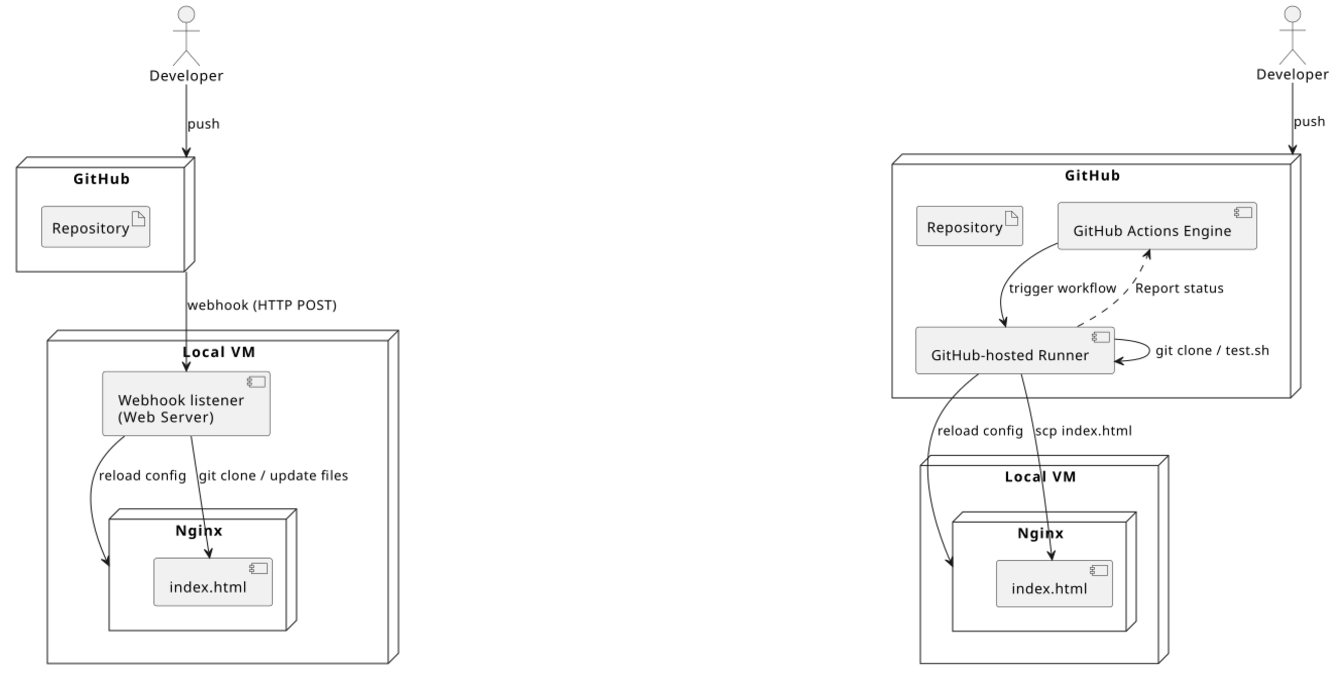
\includegraphics[width=1\textwidth]{media/result}
        \end{center}
    \end{frame}

    \begin{frame}{Наш pipeline — это CI/CD pipeline}
        \textbf{Поздравляем! Мы только что создали CI/CD pipeline}
        
        \vspace{0.5cm}
        
        \textbf{CI/CD} — собирательный термин для автоматизации задач разработки:
        \begin{itemize}
            \item \textbf{CI} — Continuous Integration (непрерывная интеграция)
            \item \textbf{CD} — Continuous Deployment (непрерывное развертывание)
        \end{itemize}
    \end{frame}

    \begin{frame}{Что такое CI и CD}
        \begin{columns}[t]
            \begin{column}[t]{0.48\textwidth}
                \textbf{CI задачи это шлюзы:}
                \begin{itemize}
                    \item Линтинг
                    \item Тесты
                    \item Сканеры безопасности
                \end{itemize}
                
                \vspace{0.3cm}
                \textbf{Цель:} убедиться что код соответствует требованиям
            \end{column}
            
            \begin{column}[t]{0.48\textwidth}
                \textbf{CD задачи это преобразования:}
                \begin{itemize}
                    \item Сборка приложения
                    \item Публикация и обновление приложения
                \end{itemize}
                
                \vspace{0.3cm}
                \textbf{Цель:} изменить состояние артефакта
            \end{column}
        \end{columns}
    \end{frame}


    \begin{frame}{Что запомнить}
        \begin{itemize}
            \item CI/CD платформы решают проблемы самодельных решений
            \item CI - проверки, CD - преобразования
        \end{itemize}

        \vspace{0.5cm}

        \begin{center}
            \textbf{Вопросы?}
        \end{center}
    \end{frame}

\end{document}